%============================================================
%  A8 practical — presentation slides
%  Team chmawa (sm3035, bc654, zw499) · presented by zw499
%  Compile with:  tectonic slides.tex   (XeLaTeX under the hood)
%============================================================
\documentclass[aspectratio=169,11pt]{beamer}

\usetheme{Madrid}
\setbeamertemplate{navigation symbols}{}      % no nav clutter
\setbeamertemplate{blocks}[default]           % square-cornered blocks

\usepackage{amsmath,amssymb}
\usepackage{graphicx}
\usepackage{array}
\usepackage{booktabs}
\usepackage{tikz}
\usetikzlibrary{positioning,arrows.meta,shapes.misc}
\usepackage{xcolor}

\graphicspath{{../figures/}}

%------------------ Cambridge-blue palette ------------------
\definecolor{camblue}{HTML}{103A5C}   % deep navy — structure / bars
\definecolor{cammid}{HTML}{2A6EBB}    % mid blue — links / secondary
\definecolor{camred}{HTML}{B5121B}    % collapse / negative result
\definecolor{camgreen}{HTML}{2E7D32}  % winning result
\definecolor{camboxhd}{HTML}{A9C7E8}  % light-blue box header
\definecolor{camboxbd}{HTML}{EDF3FA}  % pale-blue box body

\setbeamercolor{structure}{fg=camblue}
\setbeamercolor{title}{fg=camblue}
% plain black frame title with a straight rule under it (no colored bar)
\setbeamercolor{frametitle}{bg=white,fg=black}
\setbeamerfont{frametitle}{series=\bfseries,size=\large}
\setbeamertemplate{headline}{}
\setbeamertemplate{frametitle}{%
  \vskip7pt\leavevmode%
  {\usebeamerfont{frametitle}\usebeamercolor[fg]{frametitle}\insertframetitle\strut}\par
  \vskip3pt{\color{camblue}\hrule height 0.9pt}
}

\setbeamercolor{author in head/foot}{bg=camblue,fg=white}
\setbeamercolor{title in head/foot}{bg=cammid,fg=white}
\setbeamercolor{date in head/foot}{bg=camblue,fg=white}

\setbeamercolor{block title}{bg=camboxhd,fg=camblue}
\setbeamercolor{block body}{bg=camboxbd,fg=black}
\setbeamercolor{block title alerted}{bg=camred,fg=white}
\setbeamercolor{block body alerted}{bg=camred!7,fg=black}
\setbeamercolor{block title example}{bg=camgreen,fg=white}
\setbeamercolor{block body example}{bg=camgreen!7,fg=black}
\setbeamercolor{alerted text}{fg=camred}
\setbeamercolor{itemize item}{fg=camblue}
\setbeamercolor{itemize subitem}{fg=cammid}
\setbeamertemplate{itemize items}[circle]     % flat pure-color bullets

\usepackage{hyperref}
\hypersetup{colorlinks=true,urlcolor=cammid,linkcolor=cammid}

%------------------ deterministic section tracker -----------
\newcommand{\currsec}{}
\newcommand{\mysec}[1]{\gdef\currsec{#1}\section{#1}}

%------------------ custom 3-box footline -------------------
\setbeamertemplate{footline}{%
  \leavevmode%
  \hbox{%
    \begin{beamercolorbox}[wd=.26\paperwidth,ht=2.6ex,dp=1.25ex,leftskip=.6em,rightskip=.3em]{author in head/foot}%
      \usebeamerfont{author in head/foot}Team \textbf{chmawa}\,$\cdot$\,zw499\hfill%
    \end{beamercolorbox}%
    \begin{beamercolorbox}[wd=.54\paperwidth,ht=2.6ex,dp=1.25ex,leftskip=.6em,rightskip=.6em]{title in head/foot}%
      \usebeamerfont{title in head/foot}\currsec\hfill%
    \end{beamercolorbox}%
    \begin{beamercolorbox}[wd=.20\paperwidth,ht=2.6ex,dp=1.25ex,leftskip=.5em,rightskip=.6em]{date in head/foot}%
      \usebeamerfont{date in head/foot}\hfill\insertframenumber\,/\,\inserttotalframenumber%
    \end{beamercolorbox}%
  }\vskip0pt%
}

%------------------ shorthands ------------------------------
\newcommand{\code}[1]{\texttt{\small #1}}
\newcommand{\pth}{\pi_\theta}
\newcommand{\pold}{\pi_{\mathrm{old}}}
\newcommand{\pref}{\pi_{\mathrm{ref}}}
\newcommand{\Var}{\operatorname{Var}}
\newcommand{\run}[1]{\textbf{#1}}
\newcommand{\good}[1]{\textcolor{camgreen}{#1}}
\newcommand{\bad}[1]{\textcolor{camred}{#1}}
\newcommand{\wb}[1]{\href{https://wandb.ai/sichengma0514-university-of-cambridge/a8-grpo/runs/#1}{\texttt{\small #1}}}

\title[GRPO on Gemma-3 · GSM8K]{GRPO Finetuning of \texttt{gemma-3-1b-it} on GSM8K}
\subtitle{A principled fix: larger groups, not a tighter KL leash}
\author[chmawa · zw499]{Zixuan Wang\, (zw499)}
\institute[Cambridge]{Team \textbf{chmawa}: sm3035 $\cdot$ bc654 $\cdot$ zw499\\[2pt]
Multi-Agent Systems \& Agentic AI --- Practical Examination}
\date{}

\begin{document}

%============================================================
\mysec{Overview}
\begin{frame}[plain]
\centering
\vspace{1.6cm}
{\color{camblue}\rule{0.92\textwidth}{1.1pt}}\\[12pt]
{\LARGE\bfseries Part I:\ \ GRPO Finetuning of\\[3pt] \texttt{gemma-3-1b-it} on GSM8K}\\[12pt]
{\color{camblue}\rule{0.92\textwidth}{1.1pt}}
\vspace{1.35cm}

{\large Zixuan Wang\ \ (zw499)}\\[6pt]
{\small Team \textbf{chmawa}:\ \ sm3035\ \ $\cdot$\ \ bc654\ \ $\cdot$\ \ zw499}\\[1.2cm]

{\footnotesize Code:\ \href{https://github.com/wdk0082/a8-grpo}{\texttt{github.com/wdk0082/a8-grpo}}\quad$\mid$\quad
W\&B:\ \href{https://wandb.ai/sichengma0514-university-of-cambridge/a8-grpo}{\texttt{a8-grpo}}}
\end{frame}

%============================================================
\mysec{I.1  Reproducing the baseline}
\begin{frame}{I.1\quad Reproducing the baseline --- the run \& patches}
\textbf{(i) The run.}\ \ Baseline reproduced as run \run{R0} (\wb{8c2785ut}): the upstream
\textbf{Tunix\,/\,JAX} GRPO pipeline (LoRA on frozen \code{gemma-3-1b-it}), commit
\code{borisbolliet/tpu-2026@77c5a67}, run with the \code{config.py} defaults --- KL-penalty weight
$\beta{=}0.08$, group size $K{=}2$ (responses sampled per prompt), the full \textbf{3364} GRPO steps
(one epoch), \textbf{$\sim$5\,h\,05\,m} wall-clock on \code{v6e-1}.
\vspace{6pt}

\textbf{Baseline patches}\ \ (fixes for what did not run as-shipped; full diff in \code{tpu-2026\_our\_changes.patch}):
\begin{itemize}
  \item TFDS's gsm8k builder crashes under protobuf 7.x once JAX imports --- we evaluate the \emph{identical} GSM8K test via an HF \code{datasets} fallback (seed 42);
  \item raised checkpoint retention (\code{SAVE\_INTERVAL\_STEPS}\,$500{\to}100$, \code{MAX\_TO\_KEEP}\,$4{\to}40$) so the best-val checkpoint survives selection (persistence, not training).
\end{itemize}
\end{frame}

%============================================================
\begin{frame}{I.1\quad Reproducing the baseline --- accuracy \& training curves}
\begin{columns}[T]
\begin{column}{0.53\textwidth}
\textbf{(ii) Held-out accuracy.}\ \ GSM8K \emph{test} (from HF), seed 42, greedy / exact-match, reported as
\textbf{($n{=}64$ / $n{=}1319$)} --- $n{=}64$ is the \code{config.py} default eval, $n{=}1319$ the full test:
\vspace{3pt}
\begin{center}\small
\begin{tabular}{lcc}
\toprule
Model / checkpoint & $n{=}64$ & $n{=}1319$ \\
\midrule
Base \code{gemma-3-1b-it}      & 45.3 & 47.4 \\
R0 best-val (step 700)         & 42.2 & 46.7 \\
R0 final (step 3364)           & \bad{0.0} & \bad{6.2} \\
\bottomrule
\end{tabular}
\end{center}
\vspace{2pt}
{\footnotesize\textbf{best-val} $=$ the saved checkpoint \emph{nearest the peak held-out validation reward} (not accuracy).}
\end{column}
\begin{column}{0.45\textwidth}
\centering
\textbf{(iii) Training curves (R0)}\\[5pt]
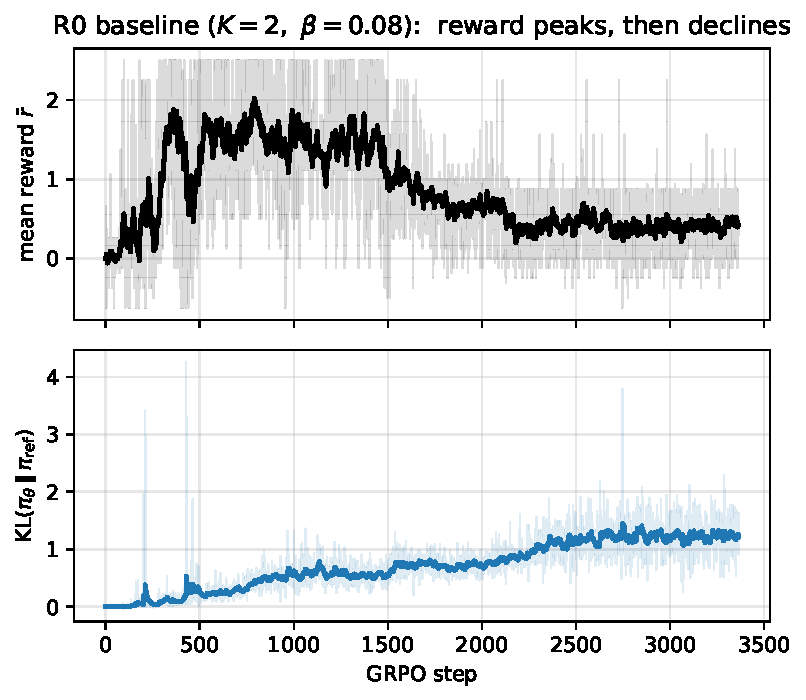
\includegraphics[width=\linewidth,height=0.74\textheight,keepaspectratio]{F1b_R0_reward_kl.pdf}
\end{column}
\end{columns}
\end{frame}

%============================================================
\mysec{I.2  Understanding the baseline}
\begin{frame}{I.2\quad Understanding the baseline}
\textbf{(a) The three policies} (all share the frozen $W_0$):
\begin{itemize}
  \item $\pth$ --- LoRA-adapted policy; the \alert{only} trainable policy ($\Delta W = \textcolor{camred}{BA}$)
  \item $\pold$ --- the rollout policy; with $\mu{=}\code{NUM\_ITERATIONS}{=}1$ (one gradient step per rollout batch), $\pold{=}\pth$ at the update
  \item $\pref$ --- frozen base Gemma
\end{itemize}
\vspace{6pt}
\textbf{(b) Group size \& advantage.}\ \ $K{=}\code{NUM\_GENERATIONS}{=}2$; Tunix \code{'grpo'} is the \textbf{standard} group-mean, std-normalised advantage over all $K$ (incl.\ $i$) --- \emph{not} leave-one-out:
\[
  \hat A_i=\frac{r_i-\bar r}{\sigma_r},\qquad
  \hat g=\frac1K\sum_{i=1}^K h_i\,\hat A_i,\qquad
  h_i=\nabla_\theta\log\pth(a_i\mid q).
\]
\end{frame}

\begin{frame}{I.2\quad Understanding the baseline}
\textbf{(c) Reward $=$ sum of four}:
\begin{itemize}
  \item \textbf{Shaping:} \code{match\_format\_exactly}, \code{match\_format\_approximately} (the \code{<reasoning>}/\code{<answer>} template)
  \item \textbf{Correctness:} \code{check\_answer} (gold match, only if the template parses) $+$ \code{check\_numbers} (any number after \code{<answer>})
\end{itemize}
\vspace{4pt}
\textbf{With the correctness reward \emph{alone}, $\sigma_r$ vanishes on most groups} --- not because the model is rarely right (base $=47\%$) but because the reward is \textbf{coarse}: at $K{=}2$ the two samples usually \emph{tie}, so
\[
  \hat A_i \;=\; \frac{r_i-\bar r}{\sigma_r} \;=\; \frac{0}{\sigma_r+10^{-6}} \;=\; 0.
\]
The dense \textbf{shaping} terms keep $\sigma_r>0$ and push toward parseable outputs (the precondition for \code{check\_answer} to vary), although they also invite reward-hacking.
\end{frame}

\begin{frame}{I.2\quad Understanding the baseline}
\textbf{(d) The clipped surrogate.}\ \ The PPO-style clip lives in Tunix's \code{GRPOLearner} (\code{tunix.rl}); the clip range is $\epsilon{=}\code{EPSILON}{=}0.2$ in \code{config.py}. \textbf{Two deviations} from the lecture form:
\vspace{3pt}
\begin{itemize}
  \item[\textcolor{camblue}{\textbf{(i)}}] \textbf{Token- vs.\ sequence-level.}\ \ The lectures clip a \textbf{per-response} ratio (one clip per whole sequence); Tunix clips a \textbf{per-token} ratio, token-by-token (a token-level objective):
  \[
    \rho_i=\frac{\pth(a_i\mid q)}{\pold(a_i\mid q)}
    \qquad\text{vs.}\qquad
    \rho_{i,t}=\frac{\pth(a_{i,t}\mid q,a_{i,<t})}{\pold(a_{i,t}\mid q,a_{i,<t})}.
  \]
  \item[\textcolor{camblue}{\textbf{(ii)}}] \textbf{The clip is \alert{inert} in this baseline.}\ \ With $\mu{=}\code{NUM\_ITERATIONS}{=}1$ (one gradient step per rollout batch) $\pold{=}\pth$, so every $\rho\equiv1$ and \textbf{nothing is ever clipped} --- the surrogate collapses to the plain policy gradient and $\epsilon$ is irrelevant. Not a \emph{contradiction} (the lecture form also reduces to this at $\mu{=}1$), but the baseline's ``clipped'' objective does no clipping until $\mu>1$.
\end{itemize}
\end{frame}

%============================================================
\mysec{I.3  Improving on the baseline}
\begin{frame}{I.3\quad Why the baseline collapses: gradient variance}
\textbf{Motivation (grounded in the lecture estimator).} The group-mean gradient has variance
\[
  \Var(\hat g) \;=\; \frac{1}{K^2}\sum_{i}(h_i-\bar h)(h_i-\bar h)^\top \;=\; O\!\left(\tfrac1K\right),
\]
\begin{itemize}
  \item \alert{Maximal at the baseline's $K{=}2$} $\Rightarrow$ noisiest updates
  \item Noisy updates let the policy chase the \textbf{dense shaping} reward (hack the format) while \textbf{true correctness decays}
\end{itemize}
\vspace{4pt}
\vspace{2pt}
{\color{camgreen}\textbf{Prediction to test:}}\ \ raising the group size $K$ shrinks $\Var(\hat g)\propto 1/K$ $\Rightarrow$ smoother updates and \textbf{milder over-optimisation}.
\end{frame}

\begin{frame}{I.3\quad The smoking gun: reward decomposition}
\begin{columns}[T]
\begin{column}{0.66\textwidth}
\centering
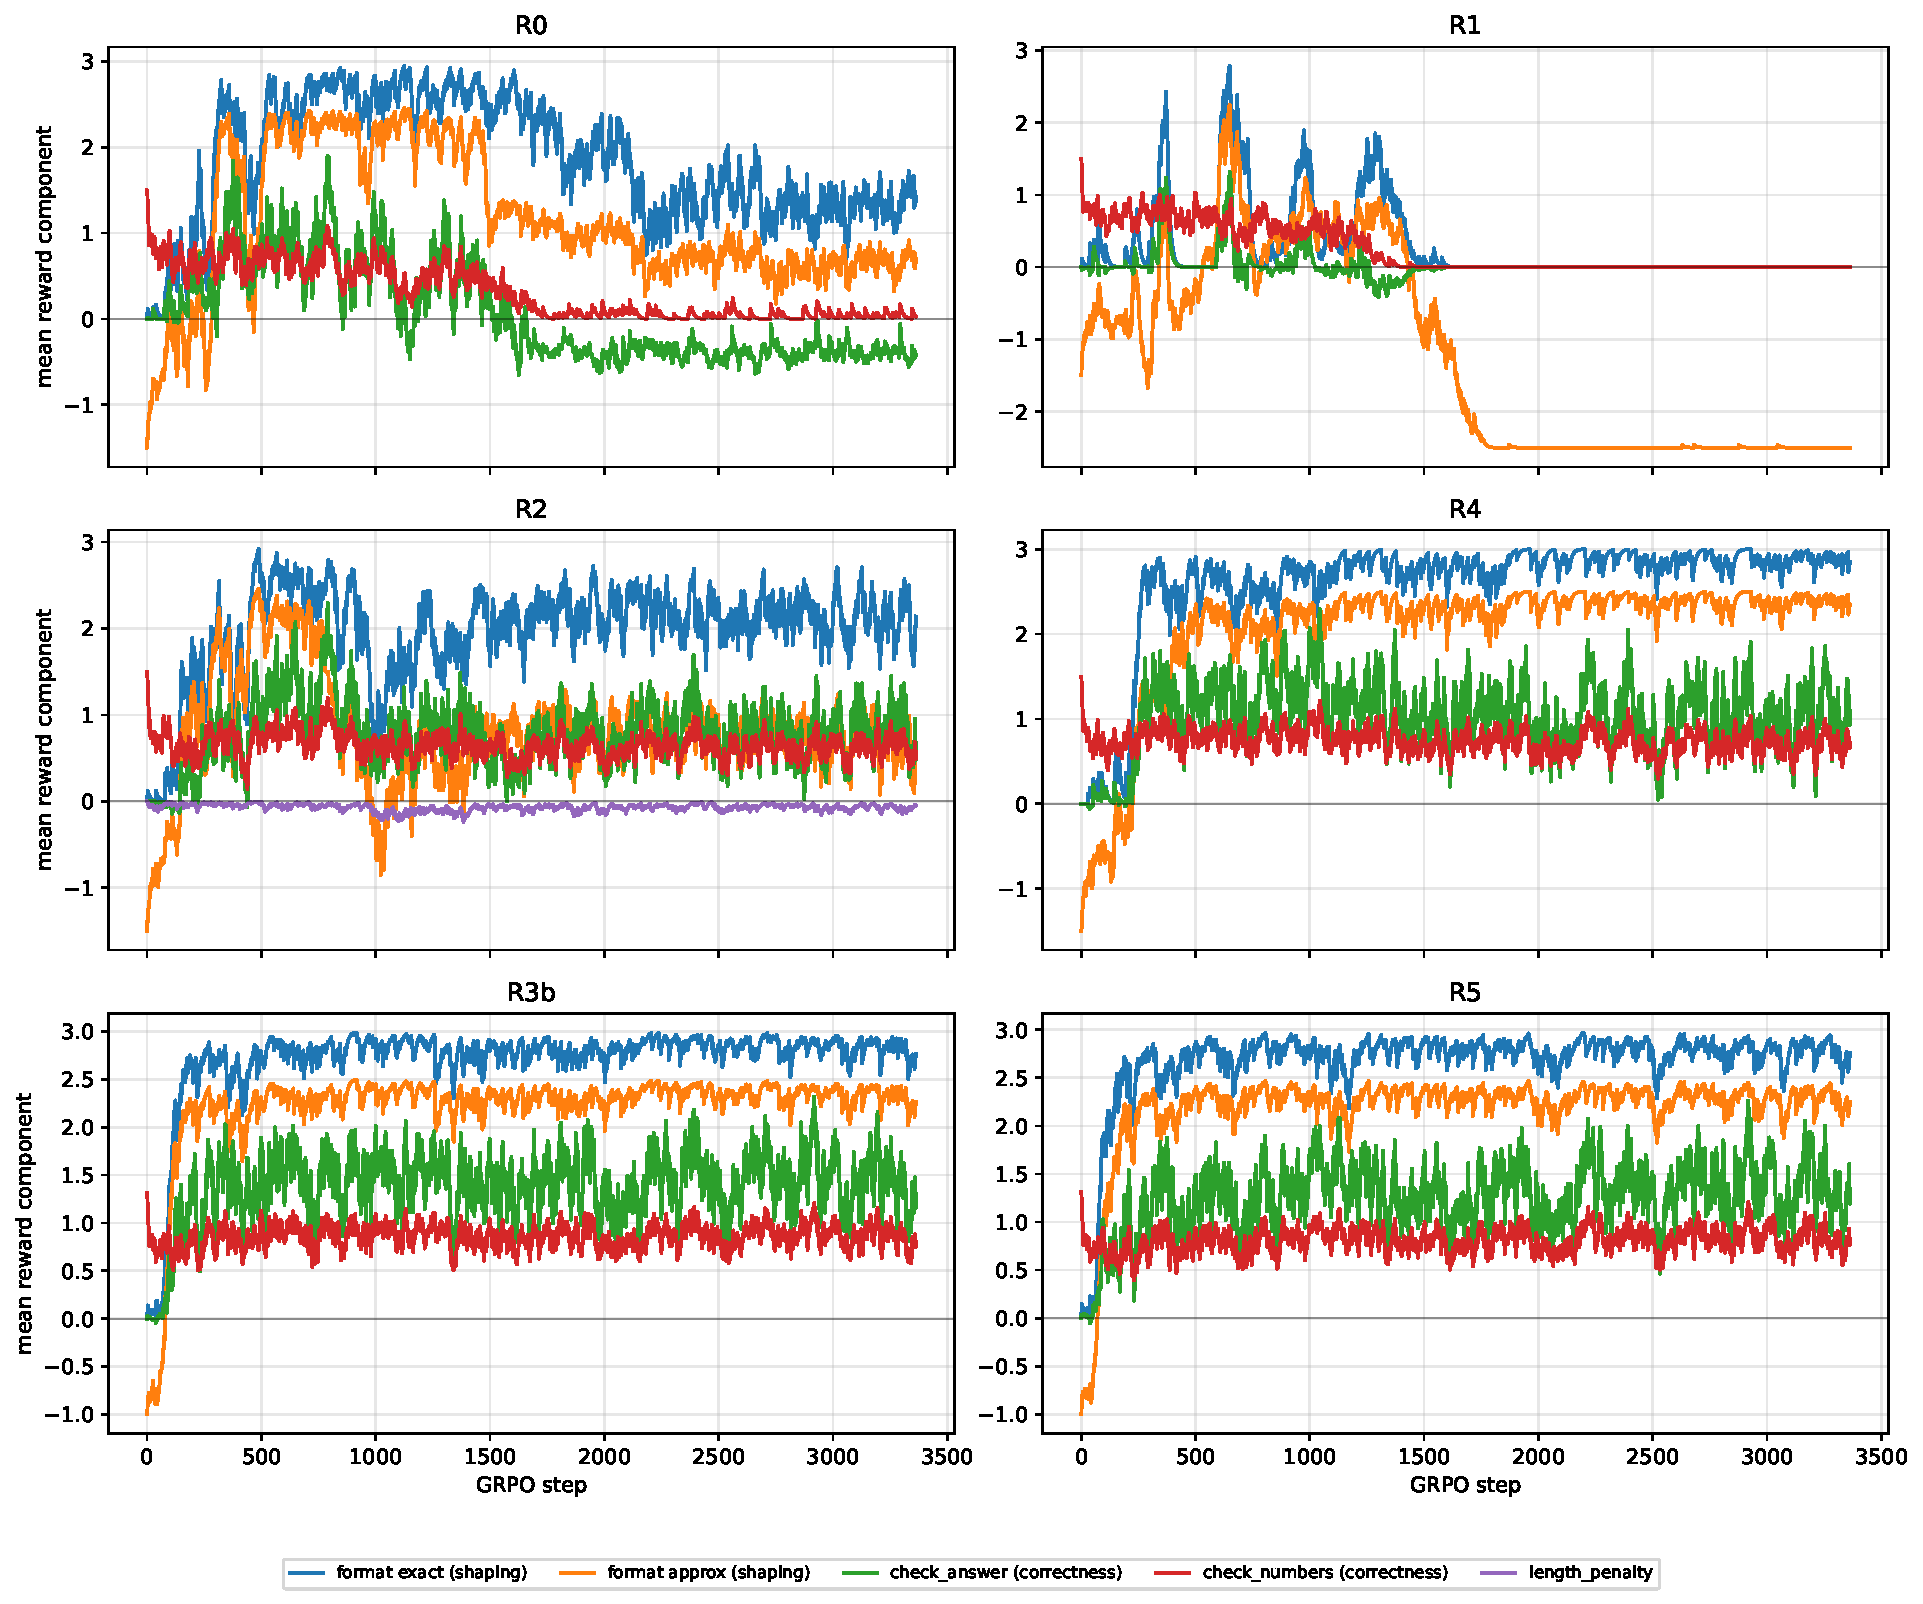
\includegraphics[width=\linewidth,height=0.82\textheight,keepaspectratio]{S1_reward_decomp.pdf}
\end{column}
\begin{column}{0.33\textwidth}
\small
In \run{R0}, the \good{correctness} reward (\code{check\_answer}) \textbf{decays} after $\approx$ step 1000 while \textbf{format-shaping stays pinned high} --- textbook reward-hacking.
\vspace{4pt}

\run{R1} ($\beta{=}0.3$) collapses entirely $\approx$ step 1700.
\vspace{4pt}

The stable $K{=}8$ runs (\run{R3b}, \run{R5}) keep correctness \emph{high throughout}.
\end{column}
\end{columns}
\end{frame}

\begin{frame}{I.3\quad Two hypotheses, one controlled $2\times2$}
\begin{columns}[T]
\begin{column}{0.54\textwidth}
\textbf{(1) Variance.} Raise $K$ $\Rightarrow$ $\Var(\hat g)\propto1/K$ $\Rightarrow$ less over-optimisation.
\vspace{4pt}

\textbf{(2) Regularisation.} The KL penalty pulls toward $\pref$; its penalised optimum is
\[
  \pi^\star(a)\;\propto\;\pref(a)\,e^{\hat A(a)/\beta}\;\xrightarrow[\beta\to\infty]{}\;\pref,
\]
so a \emph{tighter} leash (larger $\beta$) should curb the drift.
\end{column}
\begin{column}{0.44\textwidth}
\begin{block}{Design: $\beta\times K$ grid $+$ a $\beta$-axis extension}
\centering\small
\renewcommand{\arraystretch}{1.25}
\begin{tabular}{c|ccc}
      & $\beta{=}0$ & $\beta{=}0.08$ & $\beta{=}0.3$ \\ \hline
$K{=}2$ & R4 & \textbf{R0}\,(base) & R1 \\
$K{=}8$ & \textbf{R3b} & R5 & --- \\
\end{tabular}
\end{block}
\footnotesize\textbf{5 full runs}, all controlled: same data (HF GSM8K, seed 42), eval, horizon (3364 steps) and rollout RNG (\code{PRNGKey(0)}). \emph{Only the named knob changes.}
\end{column}
\end{columns}
\end{frame}

\begin{frame}{I.3\quad Training curves: reward and KL (all 5 runs)}
\begin{columns}[c]
\begin{column}{0.56\textwidth}
\centering
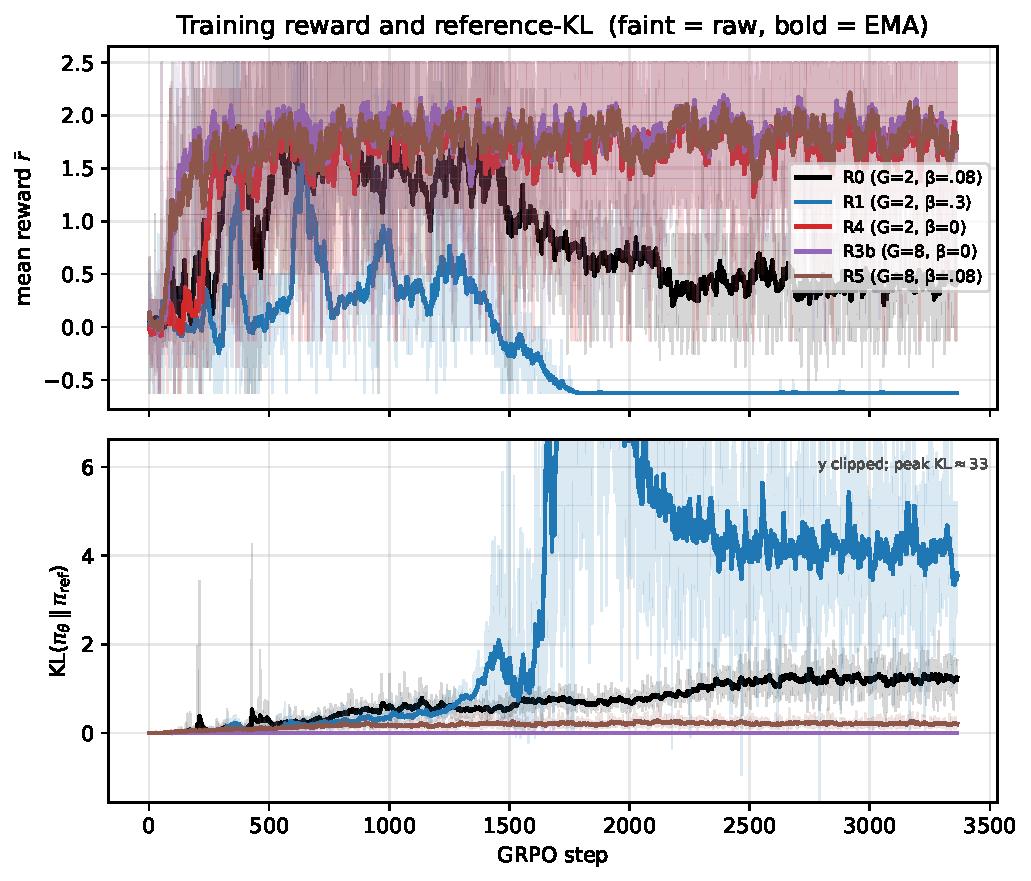
\includegraphics[height=0.80\textheight,width=\linewidth,keepaspectratio]{F1_reward_kl.pdf}
\end{column}
\begin{column}{0.42\textwidth}
\small
\begin{itemize}
  \item \bad{R0} over-optimises: reward peaks, then declines
  \item \bad{R1} ($\beta{=}0.3$) \textbf{collapses} --- KL blow-up $\approx$ step 1700
  \item \good{$K{=}8$} (R3b, R5) and R4 ($\beta{=}0$) stay \textbf{stable}
\end{itemize}
\vspace{6pt}

\textbf{\bad{Note:}}\ \ a \emph{higher} $\beta$ did \emph{not} buy a lower KL or more stability --- the opposite of prediction (2).
\end{column}
\end{columns}
\end{frame}

\begin{frame}{I.3\quad Held-out accuracy (GSM8K test, $n{=}1319$)}
\centering
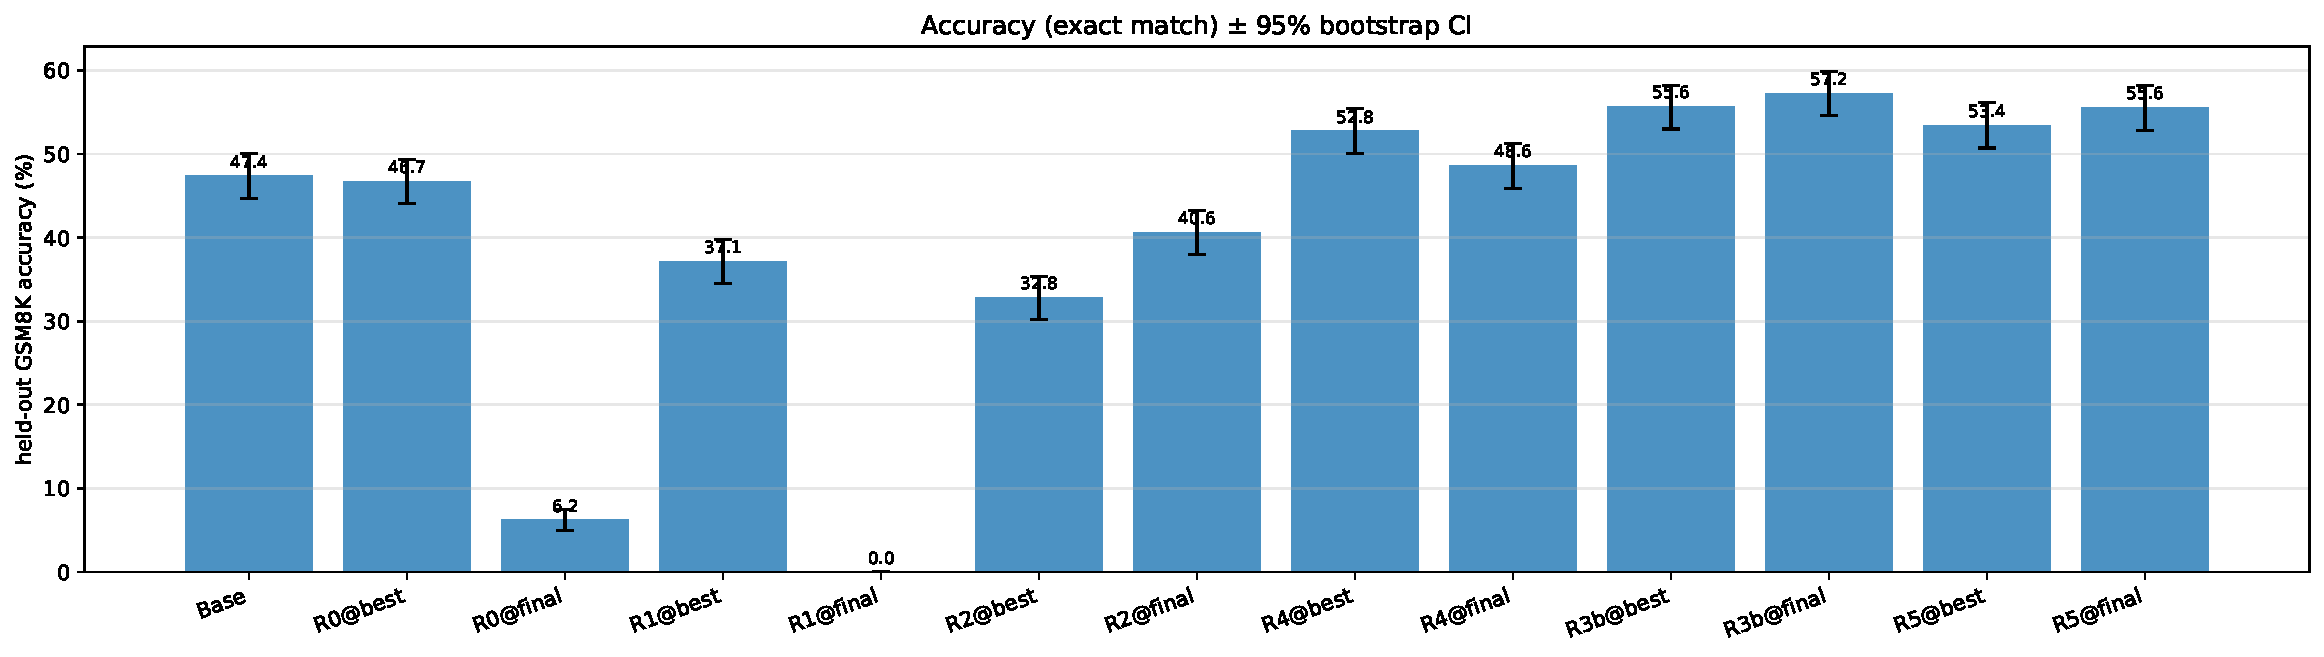
\includegraphics[width=0.96\linewidth]{F2_accuracy.pdf}\\[2pt]
\begin{columns}[T]
\begin{column}{0.62\textwidth}
\small
\begin{itemize}
  \item \good{\textbf{R3b} ($K{=}8,\beta{=}0$): \textbf{57.2\%} final, $+9.9$\,pp over base} --- best model; paired 95\% CI excludes 0
  \item Both $K{=}8$ runs beat base; each beats its matched $K{=}2$ run
\end{itemize}
\end{column}
\begin{column}{0.36\textwidth}
\small
\begin{itemize}
  \item \bad{R0 final $\to$ 6.2\%}; \bad{R1 final $\to$ 0.0\%} (below base --- a clean negative result)
\end{itemize}
\end{column}
\end{columns}
\end{frame}

\begin{frame}{I.3\quad Collapse lives in one corner: $K{=}2,\ \beta>0$}
\begin{columns}[c]
\begin{column}{0.52\textwidth}
\centering
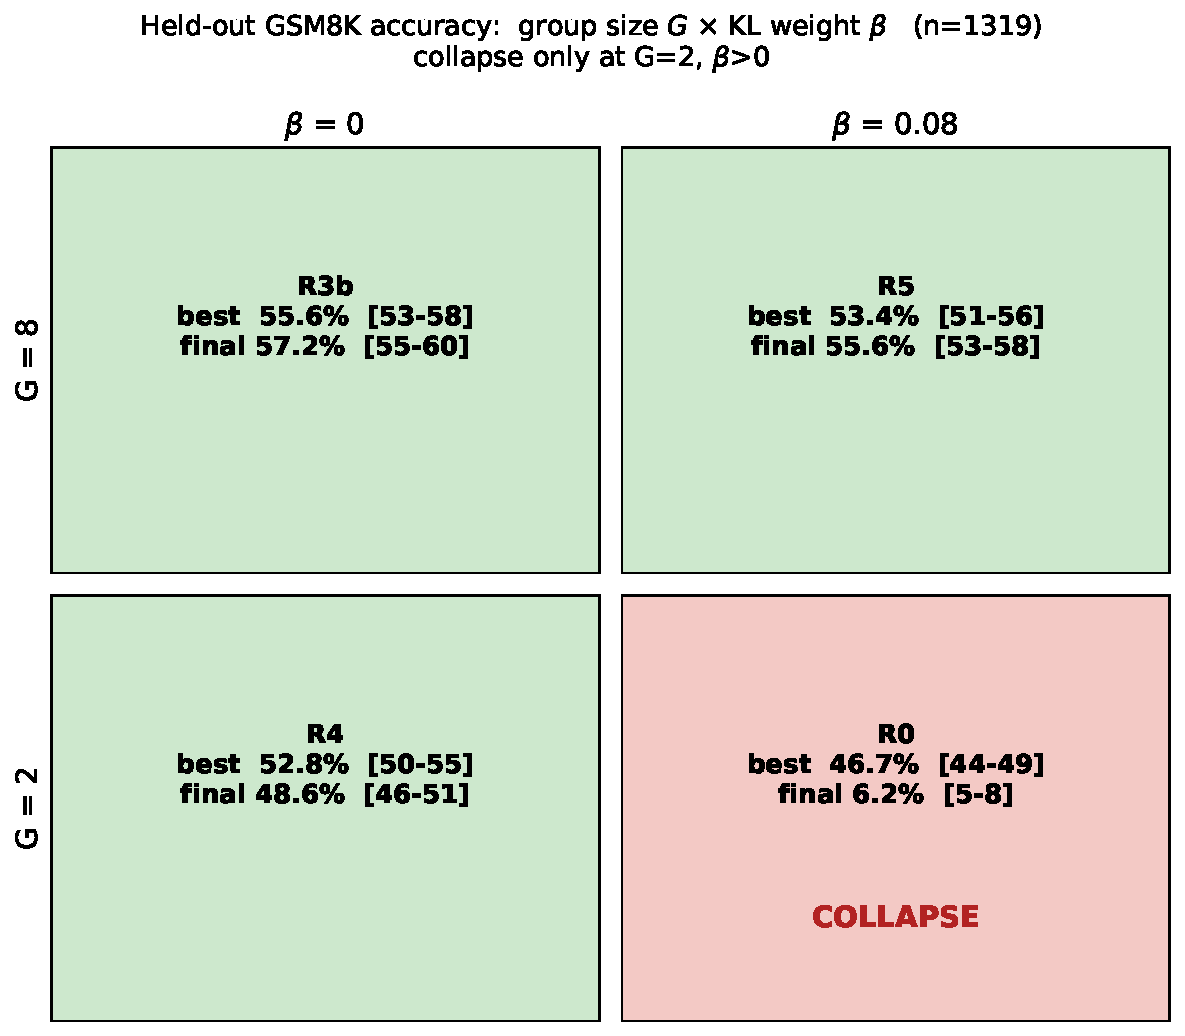
\includegraphics[height=0.76\textheight,width=\linewidth,keepaspectratio]{F4_2x2_GxB.pdf}
\end{column}
\begin{column}{0.46\textwidth}
\small
\begin{itemize}
  \item Collapse occurs \alert{only} at $K{=}2,\ \beta>0$ (R0)
  \item $K{=}2$ \textbf{peaks then degrades} (R4 $52.8\!\to\!48.6$; R0 collapses)
  \item $K{=}8$ \textbf{improves monotonically} to the final step
\end{itemize}
\vspace{6pt}

{\color{camgreen}\textbf{$\Rightarrow$}}\ \ Over-optimisation is a \textbf{$K{=}2$ phenomenon} --- exactly what the lower $\Var(\hat g)$ predicts.
\end{column}
\end{columns}
\end{frame}

\begin{frame}{I.3\quad Diagnostic --- the cost of $K{=}8$: group degeneracy}
\begin{columns}[c]
\begin{column}{0.60\textwidth}
\centering
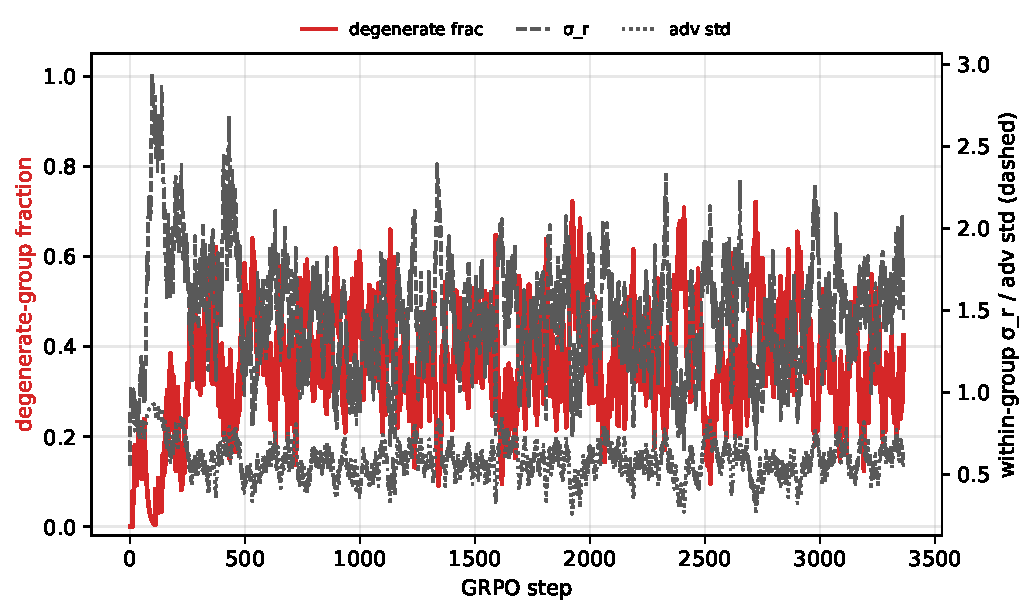
\includegraphics[width=\linewidth,height=0.82\textheight,keepaspectratio]{S3_group_degeneracy.pdf}
\end{column}
\begin{column}{0.38\textwidth}
\small
At $K{=}8$, about \textbf{a third of groups are degenerate} --- all $K$ rewards equal $\Rightarrow$ \textbf{zero advantage}, wasted samples (the known dead-group / effective-sample-size failure mode).
\vspace{6pt}

Yet within-group $\sigma_r$ \textbf{holds $\approx1.5$} (steady, \emph{not} $\to0$).
\vspace{6pt}

The net effect is still \good{$+8$--$10$\,pp}.
\end{column}
\end{columns}
\end{frame}

\begin{frame}{I.3\quad Findings vs.\ the theory}
\begin{columns}[T]
\begin{column}{0.5\textwidth}
\begin{exampleblock}{Prediction (1) \textbf{holds}}
$K{=}8$ is the winning intervention. \textbf{Variance reduction} (group size) drives the $+8$--$10$\,pp; over-optimisation is confined to $K{=}2$.
\end{exampleblock}
\end{column}
\begin{column}{0.5\textwidth}
\begin{alertblock}{Prediction (2) \textbf{contradicted}}
The tighter KL leash did \emph{not} help: $\beta{=}0$ beats $\beta{=}0.08$ at $K{=}2$; $\beta{=}0.3$ collapses \emph{faster}. At $K{=}8$ the KL weight is statistically irrelevant (R3b vs.\ R5: $+1.7$\,pp, n.s.).
\end{alertblock}
\end{column}
\end{columns}
\vspace{8pt}

\textbf{Punchline:}\ \ the cure was \textbf{variance reduction} (larger groups), \emph{not} regularisation --- echoing \href{https://arxiv.org/abs/2503.14476}{DAPO}'s removal of the KL term for long-output RL.
\end{frame}

%============================================================
\mysec{Part II  ·  Adaptive planning}
\begin{frame}{Part II\quad Adaptive planning in \texttt{cmbagent\_lg}}
\begin{columns}[c]
\begin{column}{0.605\textwidth}
\centering
\resizebox{0.98\linewidth}{!}{%
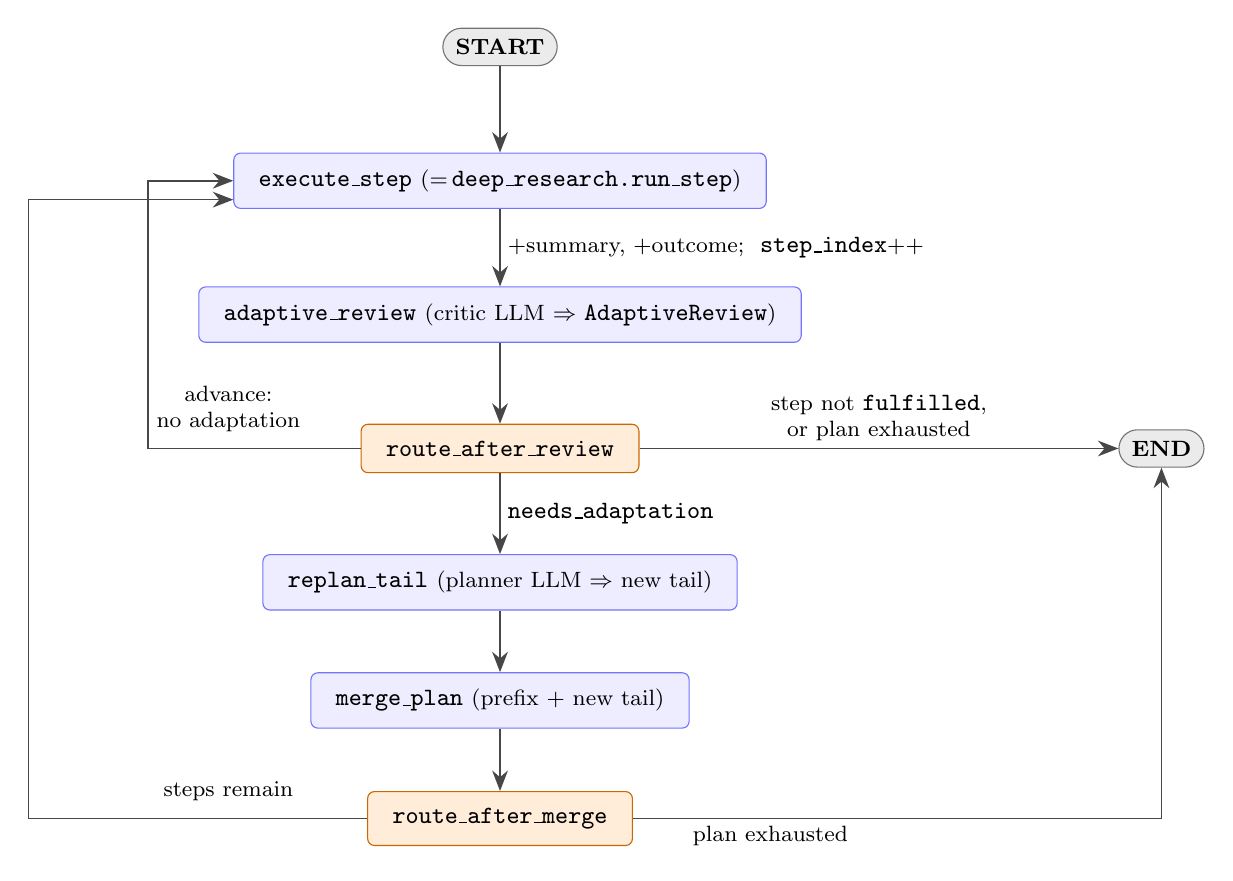
\begin{tikzpicture}[
  >={Stealth[length=2.6mm,width=2mm]}, font=\small,
  proc/.style={rectangle, rounded corners=2.5pt, draw=blue!55, fill=blue!7, align=center,
               inner xsep=9pt, inner ysep=6pt},
  rt/.style={rectangle, rounded corners=2.5pt, draw=orange!80!black, fill=orange!15, align=center,
             inner xsep=9pt, inner ysep=6pt},
  term/.style={rounded rectangle, draw=black!55, fill=black!8, align=center, inner sep=4pt, font=\footnotesize\bfseries},
  e/.style={->, semithick, draw=black!72},
  lbl/.style={font=\footnotesize, inner sep=2.5pt, fill=white},
]
\node[term] (start) at (0,0) {START};
\node[proc] (exec)   at (0,-1.7) {\code{execute\_step} {\footnotesize($=$\,\code{deep\_research.run\_step})}};
\node[proc] (rev)    at (0,-3.4) {\code{adaptive\_review} {\footnotesize(critic LLM $\Rightarrow$ \code{AdaptiveReview})}};
\node[rt]   (r1)     at (0,-5.1) {\code{route\_after\_review}};
\node[proc] (replan) at (0,-6.8) {\code{replan\_tail} {\footnotesize(planner LLM $\Rightarrow$ new tail)}};
\node[proc] (merge)  at (0,-8.3) {\code{merge\_plan} {\footnotesize(prefix $+$ new tail)}};
\node[rt]   (r2)     at (0,-9.8) {\code{route\_after\_merge}};
\node[term] (end)    at (8.4,-5.1) {END};

\draw[e] (start) -- (exec);
\draw[e] (exec)  -- (rev)  node[lbl,midway,right]{$+$summary, $+$outcome;\ \ \code{step\_index}{+}{+}};
\draw[e] (rev)   -- (r1);
\draw[e] (r1)    -- (replan) node[lbl,midway,right]{\code{needs\_adaptation}};
\draw[e] (replan)-- (merge);
\draw[e] (merge) -- (r2);
\draw[e] (r1.east) -- (end.west) node[lbl,midway,above,align=center]{step not \code{fulfilled},\\ or plan exhausted};
\draw[e] (r2.east) -| (end) node[lbl,pos=0.13,below]{plan exhausted};
\draw[e] (r1.west) -- ++(-2.7,0) |- (exec.west);
\draw[e] (r2.west) -- ++(-4.3,0) |- ([yshift=-2.4mm]exec.west);
\node[lbl,align=center] at (-3.45,-4.6) {advance:\\ no adaptation};
\node[lbl] at (-3.45,-9.45) {steps remain};
\end{tikzpicture}}
\end{column}
\begin{column}{0.375\textwidth}
\footnotesize
\textbf{Walkthrough.}
\begin{itemize}
  \item \textbf{Triggers a revision:} \code{adaptive\_review} (critic LLM) sets \code{needs\_adaptation}; the router replans \emph{iff} the step was \code{fulfilled}, the plan is \emph{not} exhausted, \emph{and} adaptation is needed.
  \item \textbf{What may change:} \emph{only} the \textbf{tail} (unrun steps); \code{merge\_plan} $=$ prefix $+$ new tail.
  \item \textbf{Held fixed:} the completed prefix, its summaries / outcomes, and \code{step\_index}.
  \item \textbf{Terminates:} when a step is not \code{fulfilled} or the plan is exhausted.
\end{itemize}
\end{column}
\end{columns}
\end{frame}

\begin{frame}{Part II\quad Problems $\rightarrow$ proposed fixes}
\small
\renewcommand{\arraystretch}{1.35}
\begin{tabular}{@{}>{\raggedright\arraybackslash}p{0.445\linewidth}@{\ $\rightarrow$\ }>{\raggedright\arraybackslash}p{0.445\linewidth}@{}}
\toprule
\multicolumn{1}{@{}c}{\textbf{\bad{Problem}}} & \multicolumn{1}{c@{}}{\textbf{\good{Fix}}}\\
\midrule
\textbf{P1 Termination not \emph{guaranteed}} --- the replanned tail can grow unboundedly; no monotone-decreasing quantity; \code{recursion\_limit} \emph{raises}, not finishes.
& Thread a \textbf{revision budget / max-steps}; routers finish gracefully; reject over-long tails. \emph{(A hard cap can truncate a genuine expansion.)}\\
\textbf{P2 Adaptation only on \emph{success}} --- a \code{fulfilled=False} step routes straight to END; no retry or route-around.
& Add a \textbf{recovery / repair path} on failure with a per-step retry budget. \emph{(Needs a recoverable-vs-fatal flag.)}\\
\textbf{P3 Replanned tail \emph{bypasses} the reviewer} that gates the initial plan --- \code{merge\_plan} splices it unchecked.
& Route \code{new\_tail} through the \textbf{existing \code{plan\_reviewer}} for one critique round. \emph{(One extra reviewer call.)}\\
\textbf{P4 Partial-state feedback at unconditional cost} --- sees only the \emph{last} step (Markov); fires every step.
& \textbf{Full-history, gated} review --- cheap model / skip when no downstream impact. \emph{(Gate conservatively.)}\\
\bottomrule
\end{tabular}
\end{frame}

\end{document}
